\begin{document}


\section{Ej1 Mealy}
\subsection{Análisis y planteo}
Para lograr la maquina de estados deseada mediante la implementaci\'{o}n de Mealy se analizo el problema en etapas. En primer lugar se plantearon los estados necesarios, las transiciones de los mismos y las salidas correspondientes a cada transición mediante un grafo. A continuación, se volcaron los estados y transiciones obtenidos del grafo en una tabla.Finalmente, se utilizo dicha tabla para obtener la tabla de verdad correspondiente al bloque de entrada de lógica combinacional tanto como para el bloque de salida. Con dichas tablas se procedió a utilizar el método de minimizaci\'{o}n por mapas de Karnaugh para conseguir la solución menor costo del problema.
\subsection{Diagrama de estados}
A continuación se presenta el diagrama de los estados,transiciones y salidas correspondientes a cada salida para la maquina de estados correspondiente al control de los niveles de agua:
\begin{center}
\begin{figure}
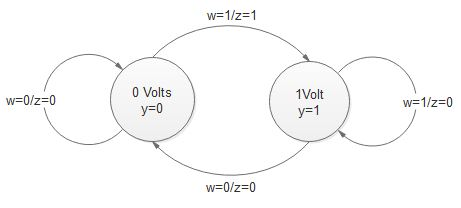
\includegraphics[scale=0.5]{Imágenes/DiagramaDeEstados.JPG} 
\caption{Diagrama de estados de la FSM}
\end{figure}
\end{center}
En el diagrama anterior la letra w simboliza el input del circuito mientras que z simboliza el output del mismo. Dichos símbolos fueron elegidos de la siguiente manera:
\begin{center}
$w=IS y z=B2B1$
\end{center}

\end{document}

